\chapter{Future colliders}
The chapter starts with a short description of the most important goals in the particle physics framework starting from the possibilities opened with the discovery of the Higgs boson.\\
It continues, in section \ref{sec:Coll-ee}, with an overview on the different projects of leptonic colliders with circular or linear structure.\\
At the end, the IDEA Detector concept is described. It is a multidetector project included in the conceptual design reports from both the two circular leptonic collider collaborations.

\section{Physics goals}
With the discovery of the Higgs boson ($H$) in 2012 by ATLAS and CMS Collaborations \cite{ATLAS_H, CMS_H}, a new era has been opened where the boson will not only be the object of researches but also the tool for new particle physics studies.\\

The total Higgs production cross section can be measured in the Higgstrahlung process ($e^+ e^- \rightarrow Z H$) looking at its presence as the recoil to the $Z$. In this way the $H$ boson is directly coupled to the $Z$ measurement.
The $H Z$ events have their recoil mass equal to $m_H$, hence Higgs bosons can be counted from the accumulation around the $H$ mass value, allowing to determine the $H Z$ cross section ($\sigma_{HZ}$).
In particular, the total cross section could be determined independently of the $H$ decay, by counting the Higgsstrahlung events characterised by a leptonic decay: $Z \rightarrow l^+ l^-$.
This method disentangled the $H$ production from its decay, providing a model-independent determination of its total width and its other couplings through branching ratio measurements with a sub-percent precision.\\

The $H$ couplings to the first Standard Model family particles (i.e. electron, quark up and quark down), because of their small masses and related decay branching ratios, will not be directly measurable at these colliders. 
However, with beam energies $\simeq 125.09\ GeV$, corresponding to the $H$ pole mass, leptonic colliders can contribute to set upper limits to the electron Yukawa coupling taking advantage from the resonant $H$ production.
Also the $t$ Yukawa and the $H$ self-couplings will not be directly measurable because their masses are too large for a kinematically open decay.
The only leptonic collider operating at $\sqrt{s} = 350\ GeV$ (FCC-ee) could exploit the $t\Bar{t}$ cross section accessing to the $t$ Yukawa with a precision of $\simeq 10\%$.\\

It is possible to predict mass and properties of the top-quark and of the bosons $Z$, $W$ and $H$ using the Standard Model. This predictions are obtained from precise measurements in the Electroweak sector and theoretical calculations.
Quantities called Electroweak Precision Observables (EWPOs) can establish the presence of new physics. For this reason EWPOs measurements represent another important component in the future colliders physics program.
The future leptonic colliders has the purpose to significantly improve in the precision (more than an order of magnitude actual one) their value and provide a broad set of EWPOs, giving access to many possible new physics sources.
Therefore, the main  studies will concern the $Z$ pole, the light neutrino species number and the $W^+W^-$ and $t\Bar{t}$ thresholds.

\section{Leptonic colliders}\label{sec:Coll-ee}

The Higgs boson can be produced in new $e^+e^-$ colliders, with high luminosity thanks to its relatively small mass.
Precise measurements of its properties, together with those of the $Z$ and $W$ bosons, will provide important tests of the SM fundamental physics principles and will be essential for the physics Beyond the Standard Model (BSM) studies.
A roadmap to achieve the results previously described is already set (see figure \ref{fig:roadmap}).
At present, the program includes 4 different leptonic collider:
\begin{itemize}
    \item the \textit{Future Circular Collider} (FCC-ee), at CERN;
    \item the \textit{Circular Electron Positron Collider} (CEPC), in China;
    \item the \textit{International Linear Collider} (ILC), in Japan;
    \item the \textit{Compact LInear Collider} (CLIC), at CERN.
\end{itemize}
In the following sections, a brief description of each one of them will be provided.

\begin{sidewaysfigure}
	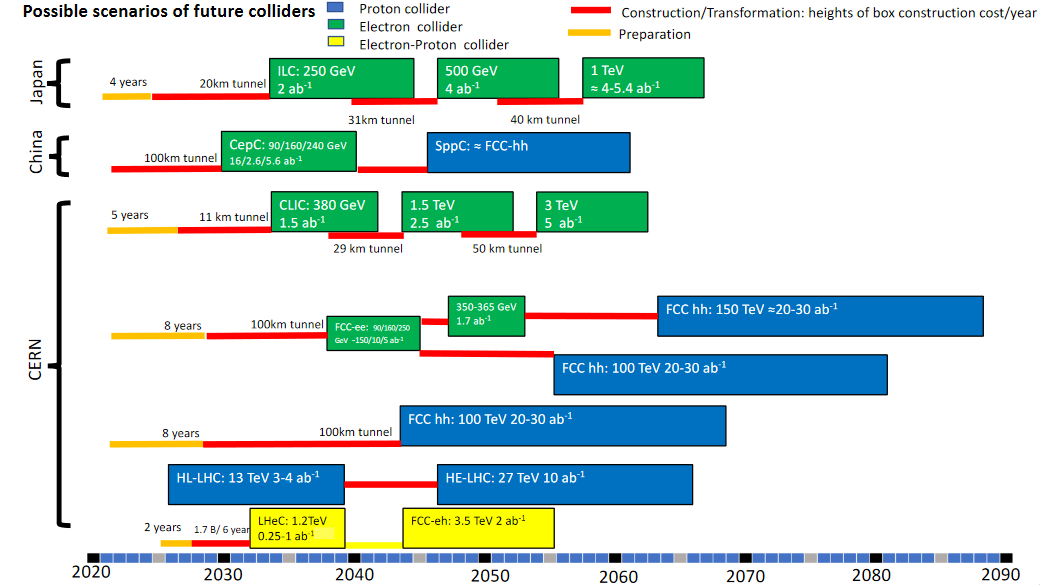
\includegraphics[width = 0.95\textwidth]{IMG/Cap1/Roadmap.png}
	\caption{Possible  timelines  of  future  colliders.  It includes $e^+e^-$ (ILC,  CLIC,  CEPC  and  FCC-ee), $pp$ (FCC-hh  and HE-LHC) and $e-p$ (LHeC and FCC-eh) machines. Image from \cite{roadmap}.}
	\label{fig:roadmap}
\end{sidewaysfigure}

\subsection*{Future Circular Collider}
A post-LHC circular collider has been proposed by the CERN with the name of Future Circular Collider (FCC) project \cite{FCC}. FCC is staged in a first lepton collider (FCC-ee) \cite{FCC-ee} phase followed by a hadron collider (FCC-hh) \cite{FCC-hh}. A common tunnel about $100\ km$ long is designed to host both of them. With this choice the same facility could also house an electron-hadron collider.\\
FCC-ee is designed to provide the highest possible statistics for the $Z$, $W$ and $H$ bosons, and $t$ quarks. For this reason FCC-ee will operate at center-of-mass energies ranging from $88$ to $365\ GeV$ in four different $\sqrt{s}$ operating points:
\begin{itemize}
    \item $\simeq 91\ GeV$, corresponding to the $Z$ pole;
    \item $\simeq 160\ GeV$, corresponding to the $W^+W^-$ production threshold;
    \item $\simeq 240\ GeV$, corresponding to the $ZH$ production threshold;
    \item $\simeq 340-365\ GeV$, corresponding to the $t\Bar{t}$ threshold.
\end{itemize}

The FCC-ee project integrates with the present CERN accelerator complex, where the injector chain makes use of a $6\ GeV$ linac, a damping ring and the CERN SPS as a pre-booster. The layout, sketched in figure \ref{fig:FCC-ee}, is designed with two different interaction points.\\
The task of increasing our knowledge of electroweak and Higgs observables by one or two orders of magnitude better than the current one sets challenging constrains to the luminosities needed. These values range from $0.2\ ab^{-1}$, for the measurement of the top-quark mass and width, to $100\ ab^{-1}$, for the measurement of the effective weak mixing angle.
These luminosities can be achieve in a reasonable amount of time only circular colliders. 

\begin{figure}
	\centering
	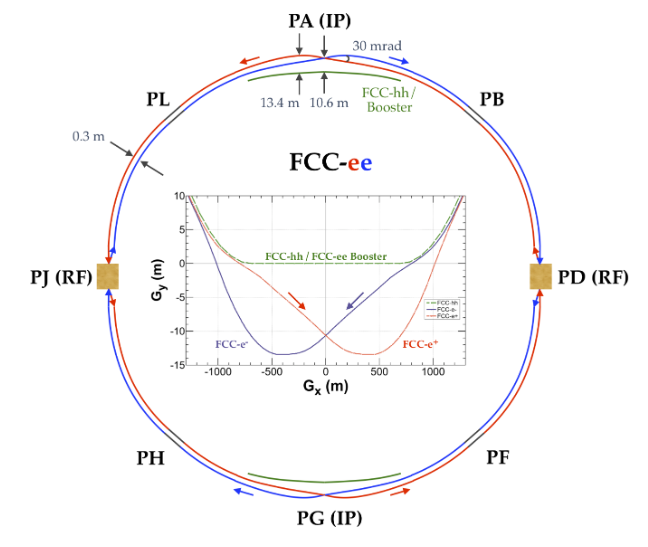
\includegraphics[width=.7\textwidth]{IMG/Cap1/FCC-ee.png}
	\caption{ Schematic view of the FCC-ee. Image from \cite{FCC}.}
	\label{fig:FCC-ee}
\end{figure}

\subsection*{Circular Electron Positron Collider}
The Circular Electron Positron Collider (CEPC) is an international project initiated and hosted by China. It is designed to operate at centre-of-mass energies of $240\ GeV$ (as $H$ factory via $e^+e^- \rightarrow ZH$), $91.2\ GeV$ ($Z$ pole) and 160 GeV ($W^+W^-$ threshold scan).\\

The collider is composed by a double ring, sketched in figure \ref{fig:CEPC} with a circumference of $100\ km$ and two interaction points. The same $100\ km$-long tunnel could also host a Super Proton-Proton Collider (SPPC), also without removing the CEPC giving the possibility of a electron-proton collision. As described in the conceptual design report \cite{CEPC_design1, CEPC_design2}, the main accelerator is preceded by a linear accelerator, a damping ring and a booster.\\
Associated to the three operating $\sqrt{s}$ values the instantaneous luminosities are expected to reach $3 \times 10^{34}$, $32 \times 10^{34}$ and $10 \times 10^{34}\ cm^{-2}s^{-1}$, respectively.
CEPC will produce, over is planned operative time, large samples (more than one million) of Higgs, one trillion of $Z$ bosons and about 100 million of $W^+W^-$ events, allowing precision measurements of their properties.\\

\begin{figure}
	\centering
	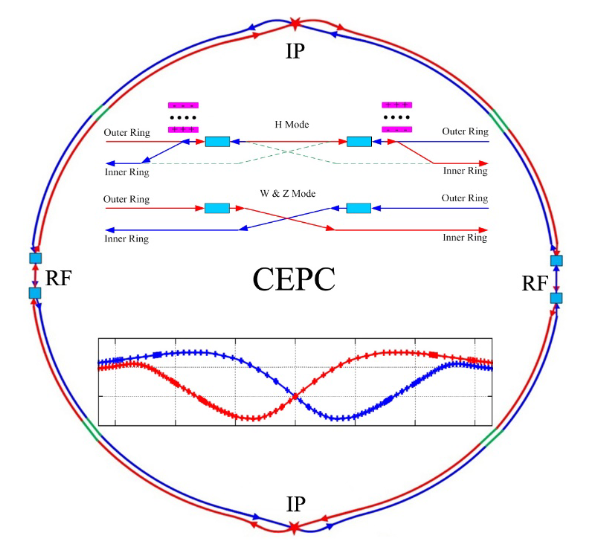
\includegraphics[width=.7\textwidth]{IMG/Cap1/CEPC.png}
	\caption{ Schematic view of the CEPC. Image from \cite{CEPC_design2}.}
	\label{fig:CEPC}
\end{figure}

According to \cite{CEPC_schedule}, the CEPC construction could be possibly start within few years and could be completed by 2030, by far the most aggressive time schedule among the big collider proposals.

\subsection*{International Linear Collider}
The ILC is an $e^+e^-$ linear collider that, at the current state (ILC250), provides a $250\ GeV$ center-of-mass energy. This value is extendible to $1\ TeV$.
The first stage of ILC has the task to measure the $H$ parameters and their model-independent determination studying the $e^+e^- \rightarrow ZH$ collision at $\sqrt{s}= 250\ GeV$.
Two energy upgrades are currently projected extending the center-of-mass energy to $500\ GeV$ and $1\ TeV$.
The higher-energy physics goals are to increase the precision on the measurement of the top-quark mass, of the top-quark electroweak couplings, of the Higgs coupling to the top quark, and of the triple-Higgs coupling \cite{ILC_global_project}.\\

It will also search for new physics hints in exotic decays of $H$ and in pair-production of weakly interacting particles. A sketch of the ILC250 is shown in \ref{fig:ILC250}.\\
The ILC accelerator is based on Super Conducting Radio Frequency (SCRF) cavities already in use in the European X-ray Free Electron Laser (E-XFEL), at DESY/Hamburg.
The estimated power consumption at the three centre-of-mass energy stages of the baseline option are \cite{ILC_design}: $122\ MW$ (at $250\ GeV$), $121\ MW$ (at $350\ GeV$) and $163\ MW$ (at $500\ GeV$). It increases to $300\ MW$ for the $1\ TeV$ option.\\
In its current state, the SCRF cavities will reach frequency values of $1.3\ GHz$ providing a gradient of $31.5-35\ MV/m$ while operating in a cryogenic infrastructure at $2\ K$.\\
The design luminosity is $1.35-1.5 \times 10^{34}\ cm^{-2}s^{-1}$, with a corresponding integrated luminosity from $400\ fb^{-1}$ (in the first years) to $2\ ab^{-1}$ (after future upgrades).
The ILC250 is $20.5\ km$ long with two main arms, mostly occupied by the electron and positron linacs, at $14\ mrad$ crossing angle. The ILC candidate site is in the Kitakami region in northern Japan.

\begin{figure}
	\centering
	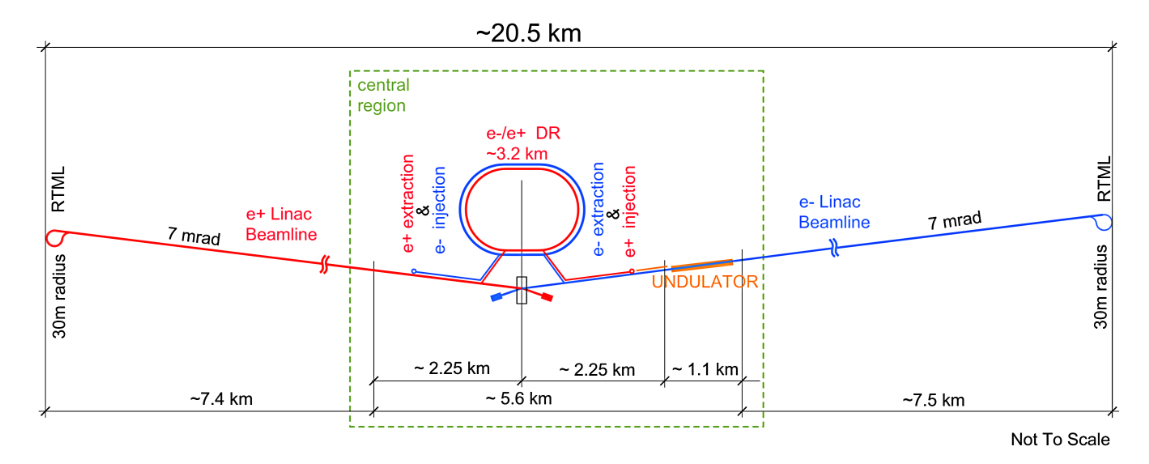
\includegraphics[width=.8\textwidth]{IMG/Cap1/ILC.png}
	\caption{Schematic layout of the ILC at 250 GeV staged option \cite{ILC_global_project}.}
	\label{fig:ILC250}
\end{figure}

\subsection*{Compact Linear Collider}
The Compact Linear Collider (CLIC) is a TeV-scale high-luminosity linear leptonic collider to be located in the CERN area. The CLIC energy stages are $\sqrt{s}= 380\ GeV$, $1.5\ TeV$ and $3.0\ TeV$, with corresponding instantaneous luminosities of $1.5$, $3.7$ and $5.9 \times 10^{34}\ cm^{-2}s^{-1}$, respectively. The site length scales, in these stages, from $11\ km$ up to $50\ km$.\\

The CLIC project, proposed in 2012 \cite{CLIC_old1, CLIC_old2, CLIC_old3} updated in 2016 \cite{CLIC_update}, will adopt a two-beam acceleration scheme as shown in figure \ref{fig:CLIC} where electrons and positrons beams are independent through the whole chain.\\
In the first stages, particles are accelerated to $9 GeV$ using a linac booster. Then they are injected in normal-conducting high-gradient $12\ GHz$ accelerating structures. The two main linacs accelerate beams exploiting normal conducting $X$-band cavities with an accelerating gradient of $100\ MV/m$. To reach these extremely high accelerating gradients a novel drive-beam scheme that uses low-frequency klystrons to generate long RF pulses and stores their energy in a long, high-current, drive-beam pulse. This beam pulse is used to generate several short pulses distributed along the main linac.

\begin{figure}
	\centering
	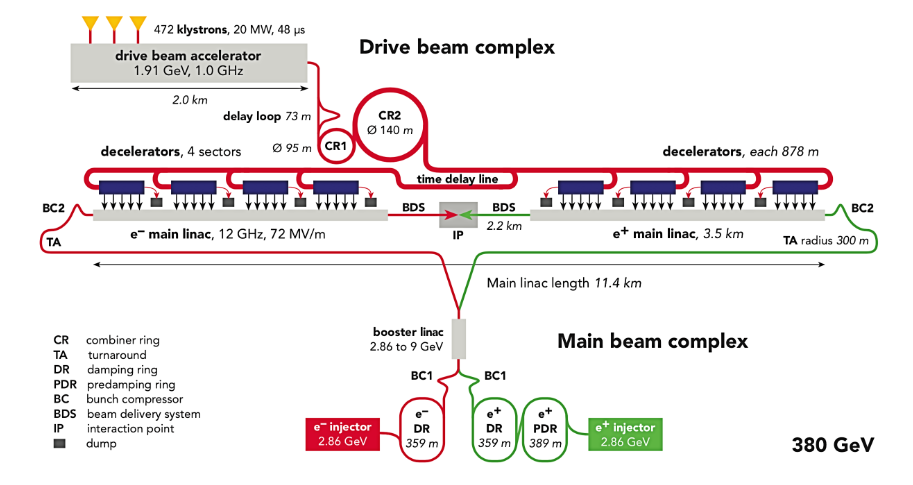
\includegraphics[width=.8\textwidth]{IMG/Cap1/CLIC.png}
	\caption{Schematic layout of the CLIC at 380 GeV staged option \cite{CLIC_img}.}
	\label{fig:CLIC}
\end{figure}

\section{IDEA Detector concept} \label{sec:Idea_project}
IDEA (Innovative Detector for an Electron-positron Accelerator) is an innovative general-purpose detector concept, designed to study electron-positron collisions in a wide energy range provided by a very large circular leptonic collider, with a typical circumference of 100 km.
The new detector concept called was proposed in 2017 and was included in conceptual design reports of both FCC-ee \cite{FCC-ee_design} and CEPC \cite{CEPC_design}.

\begin{figure}
	\centering
	\subfloat[][ Artistic view of the IDEA detector concept. \label{fig:IDEA_art1}]{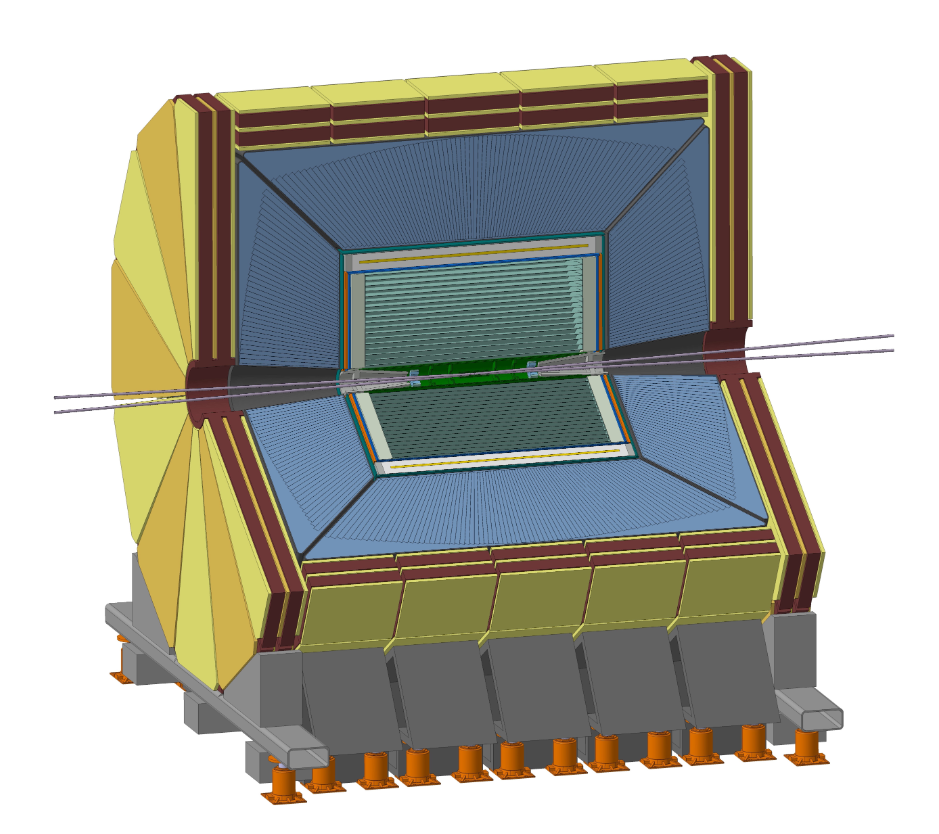
\includegraphics[width=.45\textwidth]{IMG/Cap1/IDEA_art1}} \quad
	\subfloat[][The structure and dimensions of the IDEA detector concept. \label{fig:IDEA_art2}]{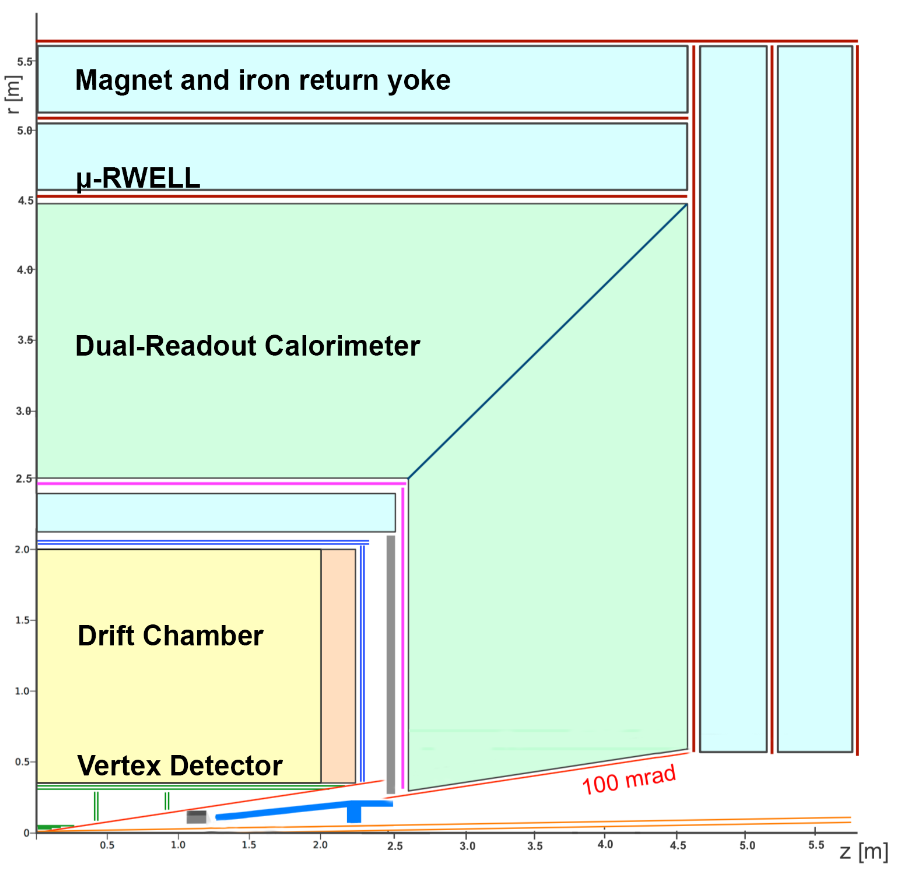
\includegraphics[width=.45\textwidth]{IMG/Cap1/IDEA_art2}}
	\caption{IDEA Detector concept.}
\end{figure}

The IDEA Detector concept is sketched in an artistic view in figure \ref{fig:IDEA_art1} and in its structure and dimensions in figure \ref{fig:IDEA_art2}. 
The overall detector is composed by a silicon pixel vertex detector, a wire chamber surrounded by a layer of silicon micro-strip detectors, a thin superconducting solenoid coil, a pre-shower detector, a dual-readout calorimeter, and muon chambers.
The most innovative elements proposed with this project are:
\begin{itemize}
  \item the ultra-light drift chamber as main tracker;
  \item the Dual-Readout (DR) fiber calorimeter.
\end{itemize}

The drift chamber technology is based on an upgrade of MEG, designed to search for the charged lepton flavor violating decay $\mu \rightarrow e^+\gamma$. The R\&D work studies the construction and operation of the MEG2 Ultra Light TIming Drift Chamber (MULTIDC) performing high momentum resolution and transparency in terms of radiation length.
The IDEA dual-readout calorimeter, on the other hand, stands on the legacy of the DREAM/RD52 Collaboration. The key point is the feasibility of dual-readout optical-fibers calorimeters to obtain high resolution in energy measurement associated to both single-hadron and hadronic jets.
All the most important parameters of the IDEA detector components are listed in table \ref{tab:IDEA_part}.\\
\begin{table}
  \centering
  \begin{tabular}{ll}
    \toprule
    Vertex technology                       & Silicon \\
    Vertex inner/outer radius (cm)          & $1.7/34$ \\
    \midrule
    Tracker technology                      & Drift Chamber and Silicon Wrapper\\
    Tracker half length (m)                 & $2.0$ \\
    Tracker outer radius (m)                & $2.0$ \\
    \midrule
    Solenoid field (T)                      & $2.0$ \\
    Solenoid bore radius / half length (m)  & $2.1/30.$ \\
    \midrule
    Preshower absorber                      & Lead \\
    Preshower $R_{min}/R_{max}$ (m)         & $2.4/2.5$ \\
    \midrule
    Calorimeter absorber                    & Copper \\
    Calorimeter $R_{min}/R_{max}$ (m)       & $2.5/4.5$ \\
    \midrule
    Overall height / length (m)             & 11/13 \\
    \bottomrule
  \end{tabular}
  \caption{Parameters of the different sub-detectors composing IDEA.}
  \label{tab:IDEA_part}
\end{table}

\subsection{Vertex detector}
The $1.5\ cm$ beam pipe is surrounded by the IDEA vertex detector composed by pixel active sensors. The structure present high-resistivity substrates architectures implementing on-pixel sparsification and data driven,time stamped readout.
The goal is a thickness of $0.15-0.30\% X_0$ per layer and a power dissipation below $20\ mW/cm^2$.
The vertex detector measures tracks of charged particles with very high precision, of the order of $3\ \mu m$ in the innermost layers, and is able to precisely reconstruct secondary vertices.
This detector will significantly benefit from the electronic and mechanical work for the ALICE ITS \cite{alice_its}, as well as of new ongoing developments, in the framework of the INFN ARCADIA R\&D project.

\subsection{Drift chamber}
The IDEA drift chamber project consist in an ultra-light Drift CHamber (DCH). Following the results obtained by the KLOE Experiment DCH \cite{KLOE} and the recent DCH for MEG2 (the MEG upgrade) \cite{MEG2}, a detector with extraordinary transparency to radiation is designed.\\

The chamber is composed by a unique cylindrical volume, co-axial to the beam axis, with an inner radius of $0.35\ m$ and an outer radius of $2\ m$, for a total length of $4\ m$. It consists of $112$ co-axial layers, at alternating sign stereo angles, grouped in $24$ identical sectors. The ammount of drift cells is $56448$ with variable size from $12.0$ to $14.5\ mm$.
The chamber is operated with a very light gas mixture of $90\%$ He - $10\%$ iC$_4$H$_{10}$ (isobutane), providing a maximum drift value of $\simeq 400\ ns$.\\
The angular coverage extends down to $\simeq 13\deg$, and could be extended with additional silicon disks between the DCH and the calorimeter end caps.\\
In the radial direction the total amount of material is of the order of $1.6\%$ of a radiation length, including inner and outer cylindrical walls and contributions from the gas mixture and the wires. On the other hand, in the forward and backward direction, the total amount of material is equivalent to about $5.0\% X_0$, including inner cylindrical walls and services end plates, instrumented with front-end electronics, signal and HV cables.\\

In the context of the MEG2 drift chamber prototypes \cite{MEG2} with $7\ mm$ cell size, a drift distance resolution of $100\ \mu m$ has been achieved with both a gas mixture and an electrostatic conditions very similar to the ones foreseen for the IDEA DCH.
Analytical calculations assuming this resolution for the DCH allow to study the momentum and angular resolution with the result shown in figure \ref{fig:DCH_res}.
The drift chamber also offers outstanding particle-identification performance using the cluster counting technology improving both spatial resolution and particle identification.

Together with the excellent expected momentum resolution, the DCH can achieve superior particle identification capabilities thanks to the cluster-counting technique. The ionization process for which electrons are released follows a Poison law, therefore by counting the total number of ionization clusters ($N_{cl}$) of a charged track one can reach a relative resolution on $N_{cl}$ that follows $1/\sqrt{N_{cl}}$. The expected performance relative to particle separation in terms of number of standard deviations as a function of the particle momentum are shown in figure \ref{fig:DCH_separation}. In this graph the solid curves refer to the cluster-counting technique, while the dashed one refers to the expected identification power for the traditional $dE/dx$ method. As it can seen, the particle separation by cluster counting is more performing in the whole range of momentum.

\begin{figure}
	\centering
	\subfloat[][Momentum and angular resolutions for $\theta= 90 \deg$ as a function of momentum. \label{fig:DCH_res}]{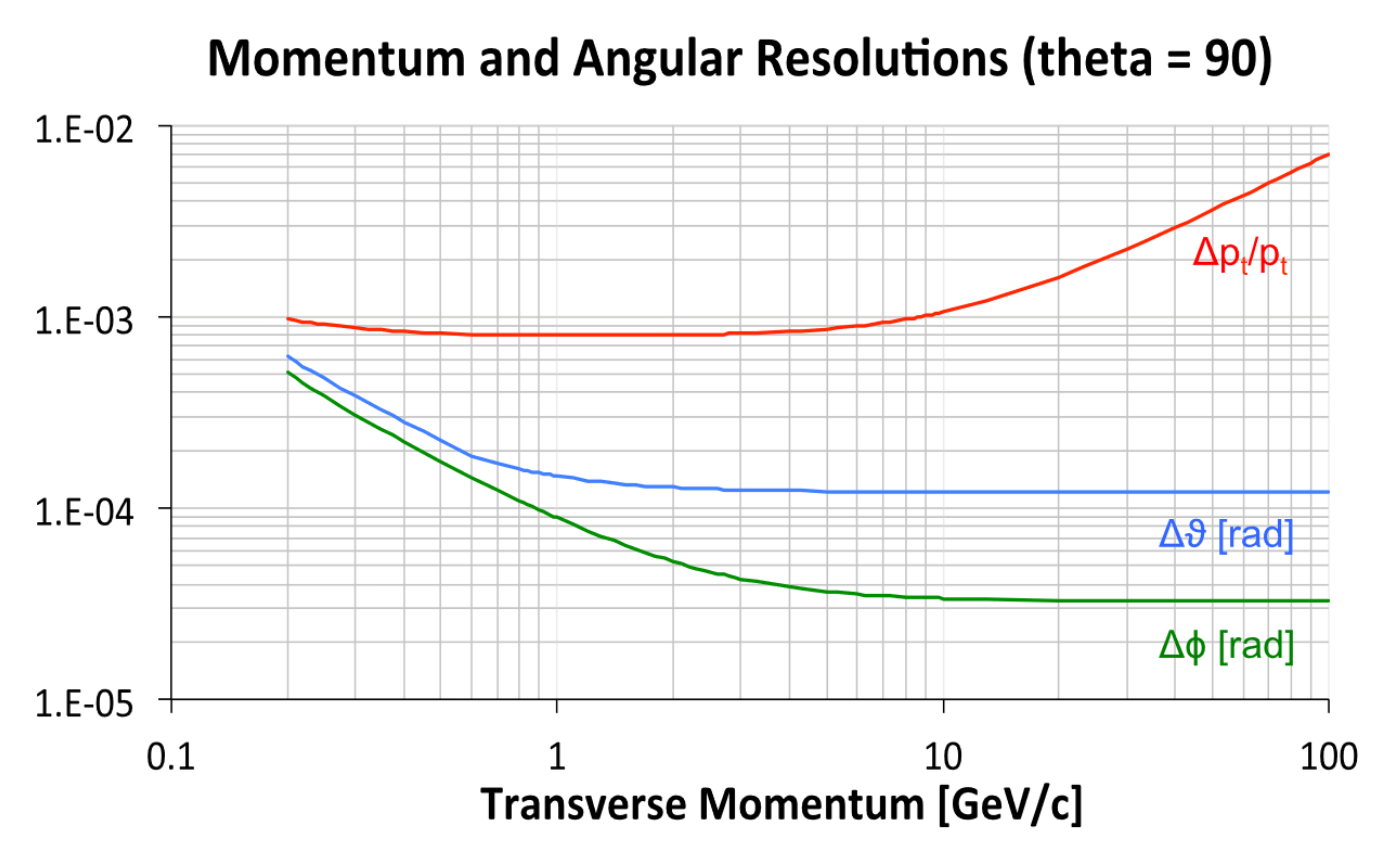
\includegraphics[width=.45\textwidth]{IMG/Cap1/DCH_res.png}} \quad
	\subfloat[][Particle type separation in units of standard deviations as a function of momentum, with cluster counting (solid curves) and with $dE/dx$ (dashed curves). \label{fig:DCH_separation}]{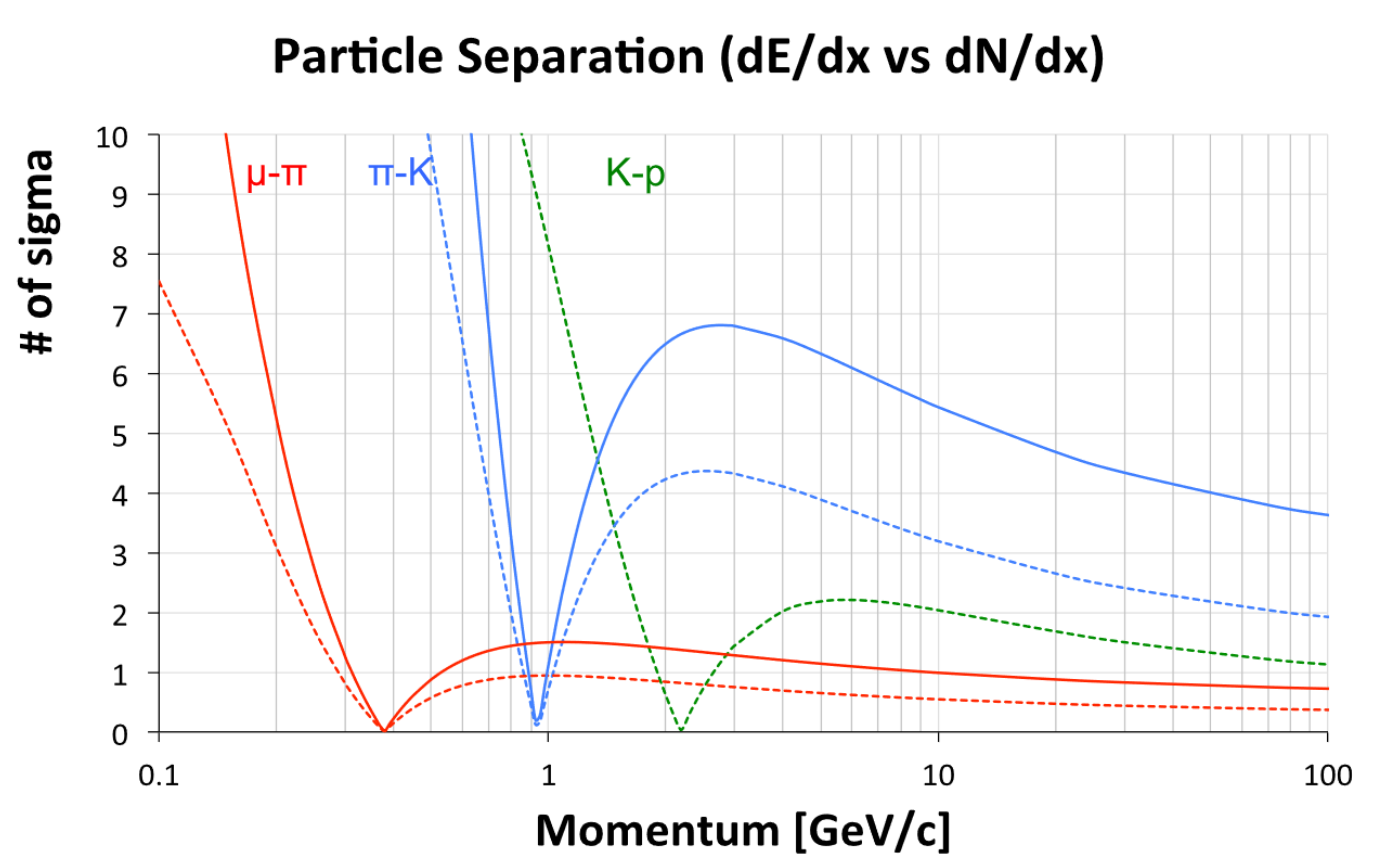
\includegraphics[width=.45\textwidth]{IMG/Cap1/DCH_separation.png}}
	\caption{IDEA ultra-light drift chamber performances \cite{FCC-ee_design}}
\end{figure}

\subsection{Magnet system}
The IDEA detector magnet is an ultra-thin and light (thus “radiation-transparent”) superconducting solenoid. It is $5\ m$ long and has an inner diameter of $4.2\ m$. equipped with a thin iron return yoke. The main feature is that the solenoid is positioned between the tracker block and the calorimeter, a solution currently employed in ATLAS.
This choice impose to keep the total thickness at $30\ cm$ level, below $1 X_0$ in terms of radiation length, but at the same time the stored energy is reduced by a factor four and the cost can be halved.
In this scenario a relatively low field of $2\ T$ can be produced.
The flux return yoke scales with the square of the coil diameter, thus with the given dimensions a yoke thickness of less than $100\ cm$ of iron is sufficient to contain the magnetic flux and to shield the muon chambers.

\subsection{Dual-readout calorimeter}
The IDEA calorimeter consist in a dual-readout projective fiber detector. It is designed starting from the studies on dual-readout performed in calorimeters as SPACAL \cite{SPACAL} and RD52 \cite{RD52}.\\
The detector is a $4\pi$ calorimeter that does not present segmentation longitudinally, but only in the direction towards the Interaction Point (IP).
The segmentation is chosen subtle to have the shower development confined in a small number of cells and most of the energy deposited in a single cell.
This highly simplifies the calibration procedures for which each cell response can be considered individually.
Considering that in accelerator-based experiments all the particle come, in good approximation, from the IP, the projective segmentation can be obtained with a tower-based structure.\\

DR calorimeters, as described in section \ref{sec:DRComp}, are composed by an absorber and two different active media to induce and transport two different signals. In the IDEA DR calorimeter copper is used as absorber, composing the structure of the towers, and filled with optical fibres as active volumes.
The possibility to independently readout each fiber with a dedicated Silicon PhotoMultiplier (SiPM), as described in \cite{Massi_tesi}, brings a series of advantages especially in terms of spatial and angular resolution removing the limitations given by the towers. Also two particle showering in the same tower, in this way, can still be identified.\\

\begin{figure}
	\centering
	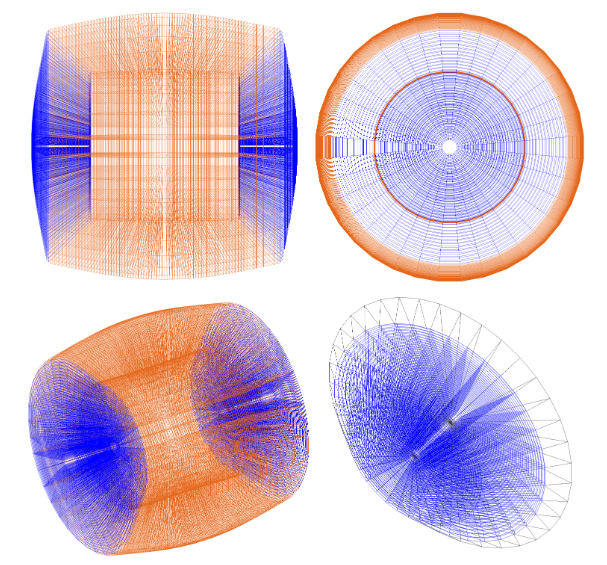
\includegraphics[width=.9\textwidth]{IMG/Cap1/DRCal_geo.png}
	\caption{IDEA dual-readout calorimetry geometry produced with GEANT4 from different angles. In orange the towers composing the barrel, in blue the ones composing the endcaps.}
	\label{fig:DRCal_geo}
\end{figure}

The geometry of the calorimeter is shown from different angles in figure \ref{fig:DRCal_geo}. To have projective towers the solution proposed is a series of truncated pyramids pointing to the IP. In such a way, each tower cover a specific region of the solid angle.\\
The cylindrical symmetry is obtained producing a rotation around the beam axis of a minimal structure called slice. A single slice cover a range of $1o\degree$ of the $\varphi$ angle, therefore $36$ of these elements cover all the calorimeter volume.
In each slice both barrel and endcaps towers are present, in particular $80$ towers for the barrel and $35$ for each endcap, with a $\theta$ coverage of $1.125\degree$ for each tower.\\
All the towers are $2\ m$ long, composed by copper and arranged to be filled by optical fibres.
The active elements are scintillating (polystyrene) and clear-plastic fibers (PolyMethyl MethAcrylate - PMMA).
The fiber diameter is $1\ mm$ thick (core + cladding) and disposed in a chess-board like geometry so that each fiber is separated from the closest ones by $0.5\ mm$ of absorber material.
This complex geometry has been reproduced within the GEANT4 simulation toolkit \cite{GEANT4} and all results in this thesis are obtained with it.

\subsection{Preshower and muon chambers}
Both the IDEA preshower and the muon chambers are based on the micro-Resistive WELL($\mu$-RWELL) technology [35]. $\mu$-RWELL chambers are compact Micro-Patter Gaseous Detector (MPGD), with a single amplification stage intrinsically spark protected.\\

A preshower detector is located in the barrel region between the magnet and the calorimeter and another one in the forward region between the drift chamber and the end-cap calorimeter.
In the barrel region, the magnet coil play also the role of of about $1 X_0$ and it is followed by one layer of MPGD chambers; a second layer of chambers follows after another $1 X_0$ of lead. In the forward region an analogue structure is built with both the $\mu$-RWELL layers preceded by $1 X_0$-long lead absorber.\\
The evaluation of the preshower performance and the single-hit-position resolution requirement are still in progress.
But with the now-a-day performances already allow to tag $\simeq 30\%$ of the $\pi^0$ from their $\gamma\gamma$ decay and provides good acceptance for photons.
This technology will perfectly match also the requirements for the IDEA muon system, providing a good tracking efficiency, high-voltage stability, a space resolution for the coordinates of a muon track of $200-300\ \mu m$ and a good time resolution thank to the fast charge amplification process.\\

Also the muon detector uses as well the $\mu$-RWELL technology but with a wider strip pitch, due to the greater dimensions. It is subdivided in three active layers at increasing distance from the vertex, and located within the iron return yoke that closes the magnetic field. Each MPGD can provide a space point with a spatial resolution of about $400\ \mu m$ in the plane perpendicular to the particle direction. Combining the three stations allows to perform standalone tracking of charged particles at $5-6\ m$ from the vertex. Such a precision also allows to identify secondary vertices that could be produced by long lived particles.